\chapter{项目设计}
\label{cha:project_design}

\section{项目描述}
本项目旨在构建一套稳定、健壮、大规模的无线Mesh网络基础设施,以支持大量的实时监控视频
数据传输。

项目基于的硬件平台为Mikrotik RB411U主板,该主板搭载Athros AR7130处理器,工作频率300MHz,
内存32MB,天线为Broadcom,工作在5GHz频段,增益12dB。该硬件平台正常通信范围为3至5km。另外,
配置Atheros AR9220无线模块,该模块对EDCA的队列机制提供硬件级支持。节点另外设计有封装外壳,
防水防爆,以适应不同的工业应用场景。

节点运行的操作系统为OpenWRT系统。基于Linux2.4.30内核,广泛使用于嵌入式无线网络设备。开发系统为
Ubuntu12.04,编译工具基于OpenWRT提供的相应硬件平台的交叉编译环境配置,引入BATMAN-adv路由
协议的包。所有使用的软件系统均来自开源项目。

实验章节中使用公开的视频序列~\cite{videos}和普通的D-link摄像头获取视频图像。

\section{BATMAN-adv路由协议}
\label{sec:3.2}
为了深入研究项目的Mesh网络特点,以便于进行深度开发,有必要首先理解Mesh网络核心协议BATMAN-adv的
技术原理。BATMAN-adv协议支持Mesh网络的自组网和数据路由两大核心功能。

\subsection{数据包类型}
BATMAN-adv协议定义了六种不同的数据包类型,用于网络的路由构建、数据包传输以及网络拓扑
可视化。网络中的节点称为Originator。这里首先对每一种数据包类型做描述。

\textbf{Originator Messages} 通常简称为OGMs,为BATMAN-adv协议的核心数据包。它用于发现
网络中的节点,每个节点通过周期性的广播OGMs申明自己的存在,以加入网络。图~\ref{fig:ogms}展示了节点广播
OGMs的过程,邻居节点接收到后更新自身的路由表并重广播出去,这样两个相互无法直接沟通的节点就能够知道彼此的存在,
从而构建有效的多跳通信路由。
\begin{figure}[H] % use float package if you want it here
  \centering
  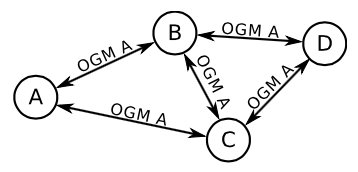
\includegraphics[width=0.5\textwidth]{OGMs}
  \caption{OGMs传播示意图,A点广播OGM,接受节点更新路由表并转发该OGM}
  \label{fig:ogms}
\end{figure}

OGMs的存在主要服务于两个目的:1)申明节点的存在,以及到达申明节点的可能的下一跳节点。
2)测量链路的质量,通过多跳重广播积累路径的整体质量。后续会详细描述。OGM包中包含如下
信息:
\begin{itemize}
\item Originator地址-用于鉴别生成该OGM的原始节点。
\item 序列号-用于链路质量度量和重复包检测。
\item 传输质量(TQ)-描述到达Originator的整条路径的链路质量。
\item 前驱节点地址-用于检测并丢弃已经广播出去的OGM。
\item TTL-用于限制OGM的最大传输跳数。
\item 网关标识-用于标识接入外网的节点。
\end{itemize}

\textbf{因特网控制报文(Internet Control Message Packet)} 简称ICMP,用以支持一部分由IP版本的ICMP提供
的特征。因为BATMAN-adv运行在mac层,因此网络中的节点不能够通过IP地址到达,因此协议提供
了mac地址到ip地址的映射机制,并基于此设计了mac地址版本的ping工具。

\textbf{单播包(Unicast Packet)} 单播数据包封装来自上层的单播数据。除了上层数据本身,单播包还
在包头中添加目的地址和TTL字段。

\textbf{分拆单播包(Fragmented Unicast Packet)} 碎片化单播数据包。BATMAN-adv封装来自上层的数据,可能超出mac层MTU长度
的限制,这就导致数据包需要被碎片化并在终点重新聚合。碎片化单播数据包除了分拆的数据外,
还需要在包头添加序号用以聚合,并添加originator的标识和碎片末尾标识。

\textbf{广播数据包(Broadcast packet)} 广播包用于向全网所有节点广播数据。除了数据部分,包头还包含
序列号,源节点地址和TTL。

\textbf{可视化数据包(Visualization packets)} 可视化数据包用于支持动态的图形化网络拓扑。用户需要先
设定其中一个节点为服务器,服务器节点会向网络中其他节点发送可视化数据包,搜集其他节点
的信息,从而构建出整体网络的拓扑图。

\subsection{节点发现}
如前所述,BATMAN-adv协议中所有节点会周期性的向其他节点广播OGMs,当一个节点接收到OGM后,
会做如下处理:
\begin{itemize}
\item[1.] 检查该OGM包中的originator是否为自身,如果是,则发送者为直接邻居,路由表做相应更新。
\item[2.] 检查该OGM包的前一跳发送节点是否为自身,如果是,表示该OGM已经处理过,直接丢弃。
\item[3.] 检查originator是否已经在路由表中存在,如果否,创建该路由表项。
\item[4.] 更新到达originator的路由表项。
\item[5.] 更新TQ和TTL值,重广播该OGM。
\end{itemize}
在此基础上,还会对路由循环和重复OGM做检查。

\subsection{链路质量估计}
\label{sec:3.2.3}
TQ值是用以估算链路质量的核心度量值,在OGM的传输过程中,TQ值逐跳计算并累计。TQ值实际上
描述了数据包在该链路上按预期到达的概率。该值存储为一个8位的值,大小位0-255。

\begin{figure}[H] % use float package if you want it here
  \centering
  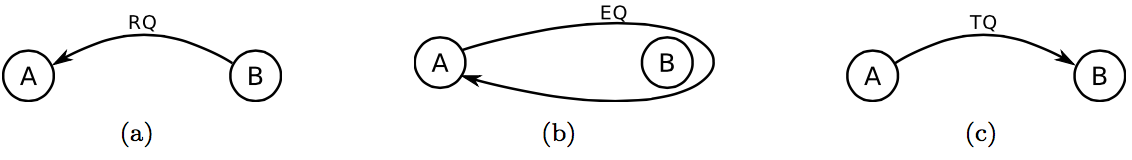
\includegraphics[width=0.8\textwidth]{TQ-RQ-EQ}
  \caption{计算TQ}
  \label{fig:TQ-RQ-EQ}
\end{figure}

\textbf{接收质量} 定义为RQ。如图~\ref{fig:TQ-RQ-EQ}(a),节点B发送OGM并被节点A接收到,A点根据来自B的OGM序列号
计算从B到达A的单向链路RQ。该过程通过一个大小为N的滑动窗口(默认大小128)实现,在该滑动
窗口中将纪录从最后接收到的OGM的序列号向前推N个对应的OGM。RQ值即为滑动窗口内序列号对应
的OGM中实际接收到的比例。

\textbf{回程质量} 定义为EQ。如图~\ref{fig:TQ-RQ-EQ}(b),节点A发出的OGM到达B后,B会重广播该OGM,A再次收到该OGM即可
计算链路的回程质量。计算类同RQ,同样通过一个纪录序列号的滑动窗口实现。

\textbf{传输质量} 定义为TQ。如图~\ref{fig:TQ-RQ-EQ}(c),传输质量指数据包从节点A发出,被节点B正确接收的概率。因为
EQ定义为数据包双向回程正确接收的概率,RQ定义为链路反向的正确接收概率,由此即可计算A点
到B点的链路传输质量TQ:
\begin{equation}
EQ=RQ*TQ
\end{equation}
\begin{equation}
TQ=\frac{EQ}{RQ}
\end{equation}


\subsection{TQ传播}
网络中的节点从OGM中可以获得前一跳节点到达目的节点的TQ值。如图~\ref{fig:TQprop}所示,A点发出OGM,
该OGM传播途径的每一个节点根据OGM中纪录的全局TQ值,结合自身邻居表存储的本地TQ值,
更新自身到达A点的TQ值,并将OGM中的TQ值同步更新,之后重广播该OGM。

\begin{figure}[H] % use float package if you want it here
  \centering
  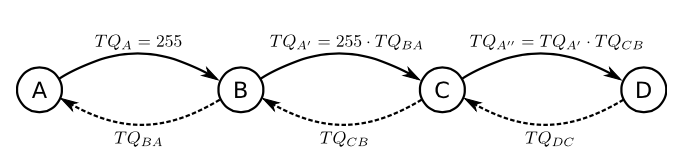
\includegraphics[width=0.7\textwidth]{TQprop}
  \caption{TQ传播}
  \label{fig:TQprop}
\end{figure}

如果节点A发出的OGM通过两条不同的路径到达某一节点,接收节点分别计算两条路径的全局TQ值,
并选择链路质量更好的那一条作为最优路由路径。每经过一次节点重广播,OGM中的全局TQ值会加
上一个惩罚值,这一实现使协议在选择时更佳倾向于选择跳数更少的路由,全局来讲,这有利于
优化信道资源的竞争。

\subsection{路由选择}
不同于很多其他协议计算整个网络的拓扑,存储到达目的节点的整条路由,BATMAN-adv仅存储到达
目的节点的最优下一跳节点。下一跳节点收到该数据包后,会继续寻找最优下一跳发送。

图~\ref{fig:routeselect}给出了一个路由决策的场景示例。节点F发送一个数据包到节点A。节点F所
知道的信息仅为到达节点A有两条有效路径,两条路径分别对应两个不同的TQ值。此时,如果途经D的路
径TQ值更高,则F选择将数据包交给D。D点经过同样的决策过程,将数据包交给C,最终由C完成最后一
跳传输。

\begin{figure}[H] % use float package if you want it here
  \centering
  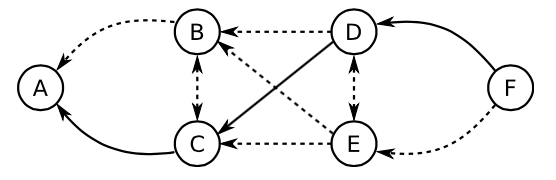
\includegraphics[width=0.6\textwidth]{routeselect}
  \caption{路由选择示例}
  \label{fig:routeselect}
\end{figure}

\section{全局QoS保障技术}
本项目的主要目标是在无线Mesh视频传输网络中提供QoS保障,保证在不同场景下,用户能够接收到流畅的视频
流数据。在第二章相关工作中已经介绍了目前该领域的研究现状,这些工作或多或少存在
大规模应用的弊端。因此本文基于全面详尽的实验,提出了一套优化整体无线Mesh视频传输网络QoS的技术方案。
整个方案分为如下三项核心创新点:

\subsection{子网信道隔离}
    无线网络中核心的技术挑战在于无线信道的开放性,这就意味着当多个设备需要发送数据时,同一时刻
只能有一个设备有效传输。虽然现在有诸如OFDM~\cite{OFDM}、MIMO
等技术来应对这一问题,但目前
市面上的硬件产品并不都能够很好的支持这些技术,因此不具有普适性。
    子网划分即将整个大的Mesh网络划分为多个子网,相邻子网间采用相互正交的信道,从而降低节点间相互
信道竞争造成的干扰。整体上提升网络的吞吐量。

\subsection{跨层视频帧权重差分}
    该方法引入802.11协议簇的QoS保障技术,该技术在系列标准的802.11e~\cite{IEEE80211e}
    子标准中规定。其核心
在于将应用层业务数据映射到不同的mac层优先队列,不同的优先队列有不同的信道接入优先级,从而保障
重要的对时延敏感的数据尽快获取信道进行传输。

\subsection{路径质量敏感的动态切换阈值}
    在移动场景下,无线Mesh网络的组网协议会面临更加严峻的挑战,尤其是高速移动的场景下,batman-adv
协议的路由切换机制存在缺陷。该部分主要工作是降低路径切换时延,并有效抑制路由震荡。
后面的章节将通过深入细致的实验验证,并设计实现解决方案。

\section{辅助模块开发}
针对不同的需求,已有无线Mesh路由协议仍然存在很多优化的空间。
为了深入的探索协议的运行机制、不同参数的影响,需要深入协议源码进行实验探究。另外,本项目
旨在搭建实际运行的系统,因此所有实验均在实际的设备上运行测量。为此,开发了手动设定固定路由
工具、外接显示模块装置、基于web端的网络可视化与诊断系统等功能模块。

\textbf{静态路由设定模块} 提供给Mesh网络管理员手动设定固定路由的工具,包括命令行即时交互接口。
这个工具可以很大程度上提升实验和网络设定的自由度。在实验中,Mesh网络可能根据协议形成固定的
拓扑结构,一旦产生外界的数据压力,拓扑结构就会变化,我们很难进行一些压力测试,比如切换条件等
一些临界状态的测试。另外在实际部署中,手动设定部分稳定链路的路由可以保障整体网络拓扑的稳定,
避免因为一些链路的抖动,造成整个网络拓扑变化频繁,影响性能。

\textbf{外接显示模块} 提供rssi轮询显示和带宽测试两项功能。正常模式下,轮询的显示邻居节点的rssi
值,当用户需要测量到达子网簇首的带宽时进行模式切换即可实时测量。

\begin{figure}[H]
  \centering
  \includegraphics[width=0.6\textwidth]{Backdesign}
  \caption{外接显示模块图示}
  \label{fig:backdesign}
\end{figure}

该模块通过硬件和软件
两部分配合实现。硬件部分采用单片机加数码管,并集成USB接口,通过USB接口直接连接到Mesh主板。
软件部分在Mesh主板运行一个后台shell进程检测USB口输入信号。正常模式下,后台进程周期性的通过
iwlist命令扫描周围邻居节点的rssi值。当用户需要测试部署位置到达子网簇首的有效带宽时,通过按
测试按键,硬件模块会通过USB接口通知后台进程进行带宽测试,然后返回测量数值显示在数码管上。

\textbf{网络可视化与诊断系统} 当网络规模达到一定规模,就很难通过终端监控网络拓扑、网络
性能和网络中节点健康状况。为了更好的提供对于大规模网络的监控和维护等功能,我们开发了基于
web端的可视化及诊断系统。我们在一台服务器上搭建Apache服务端,提供web服务,同时该服务器连接
Mesh网络中的某一个开通了可视化管理功能的节点,开通了可视化管理功能的节点使用可视化数据包
获取网络拓扑信息,作为可视化服务器的角色存在与Mesh网络中。客户端通过Apache提供的端口登录
web服务,web页面实时显示网络的拓扑形态,每条链路的链路质量、节点各项性能参数。
web界面如图~\ref{fig:diagnose_web}所示。

\begin{figure}[h]
  \centering
  \subcaptionbox{}
      {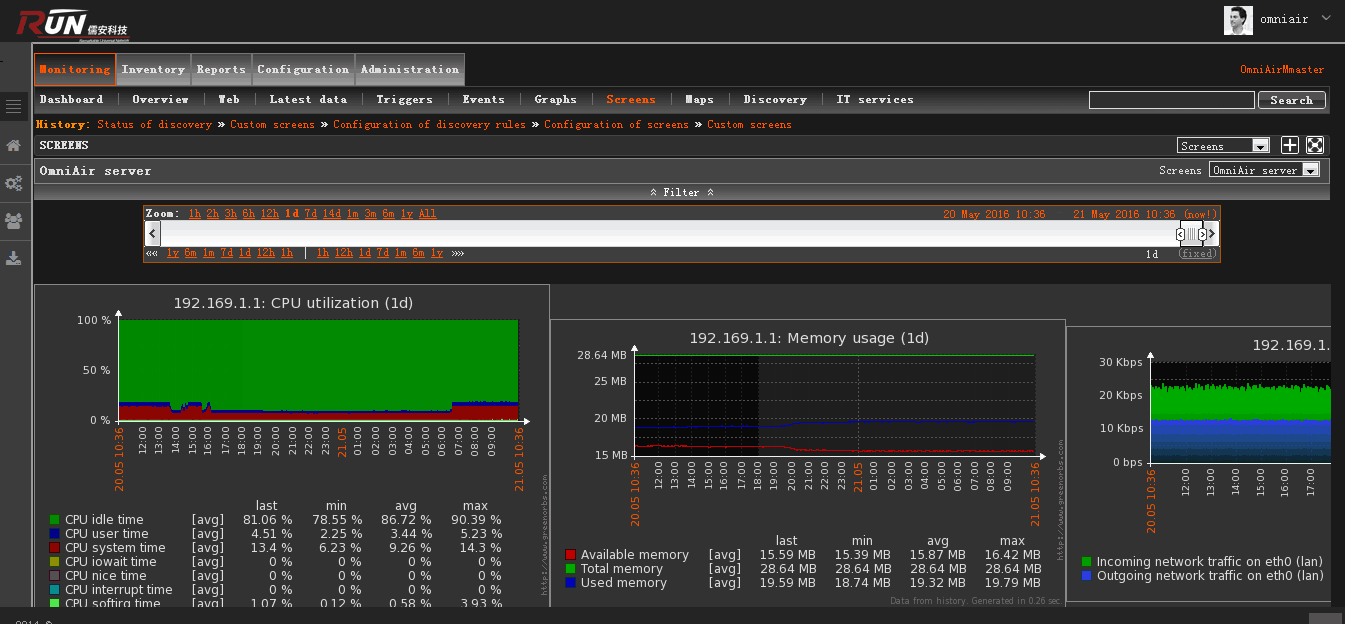
\includegraphics[height=4.5cm]{Diagnose_web1}}
  \hspace{1em}
  \subcaptionbox{}
    {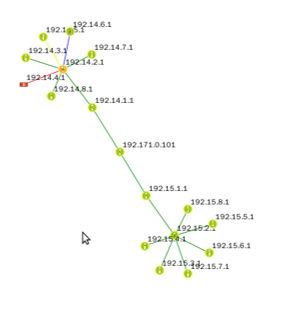
\includegraphics[height=4.5cm]{Diagnose_web2}}
  \caption{诊断系统展示}
  \label{fig:diagnose_web}
\end{figure}













